\chapter{Importing Mesh From Third Party Software in OpenFOAM}
\thispagestyle{empty}
\label{sec:chap15}
\newcommand{\LocCHonefivefig}{\Origin/CHAPTERS/chap15/figures}

OpenFOAM can be used for creating and meshing geometrical shapes like Box, Pipe. When dealing with complex geometries like a turbine blade, aircraft,
ship etc, we cannot use the blockMesh utility. In such cases it is always better to create the geometry and mesh in dedicated CAD and Meshing softwares 
and solve those usiing OpenFOAM. As a prerequisite it is expected the user should have knowledge about creating geometry and generating mesh in softwares
like Gmabit, Gmsh, Salome, ICEM etc. This chapter deals with the steps involved in importing mesh files in OpenFOAM using different mesh conversion tools.

\section{Geometry}

We will use the above problem of Flow over a square cylinder as an example for importing mesh file in OpenFOAM. Here we have a square cylinder
of length 1m and height 1 m. Inlet velocity is set at 1 $\frac{m}{s}$ for Reynolds number (Re) 100. The size of the domain choosen is 60 m by 40 m.
The boundary conditions are as shown in the , Fig \ref{square} below.

\begin{figure}[t]  
\centering  
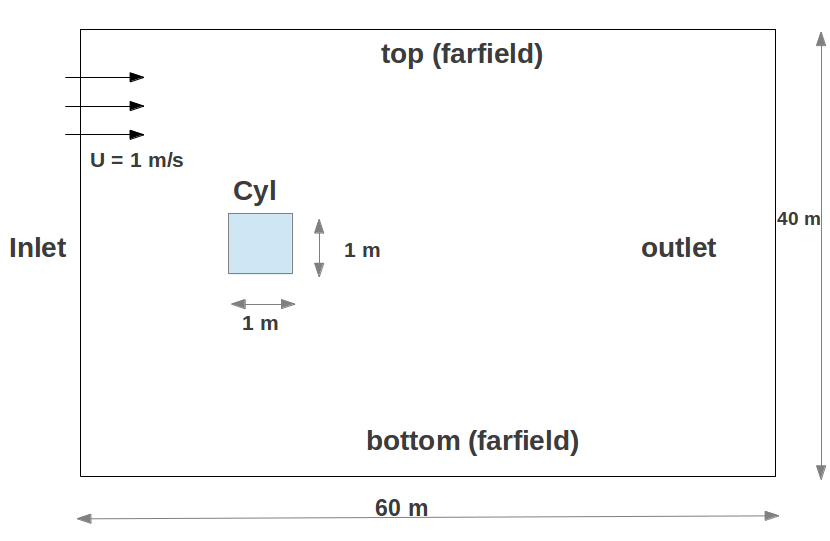
\includegraphics[width=\lgfig]{\LocCHonefivefig/square.png}
\caption{Flow over square Cylinder}
\label{square}  
\end{figure}

\section{Meshing}

We have generated a hexhedral mesh for the above geometry with 40000 cells and saved the mesh file as cylmesh.msh. 
The mesh generated is as shown below, Fig \ref{mesh} 

\begin{figure}[h]  
\centering
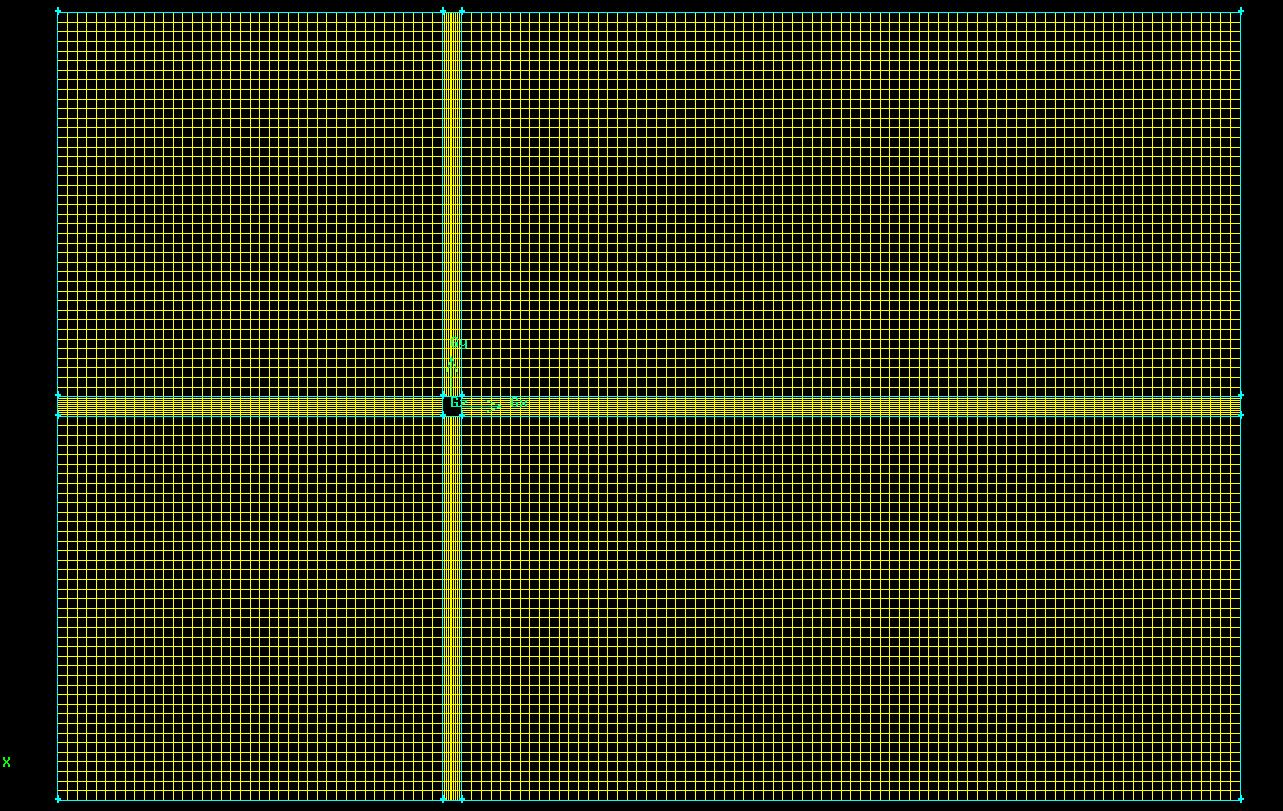
\includegraphics[width=\lgfig]{\LocCHonefivefig/cylmesh.jpeg}
\caption{Mesh}
\label{mesh}
  
\end{figure}

\section{Importing the mesh file}

In incompressibel solvers go to icoFoam and create a solver inside it by the name \textbf{cylinder}. Now go inside the cavity case and copy the 
\begin{itemize}
\item 0
\item system
\end{itemize}

\flushleft folder and paste it inside the cylinder folder. Please make a not here that we do not need the \textbf{constant} folder here. After this copy the 
cylmesh.msh mesh file create earlier and paste this inside this folder. Thus the our case file is now ready. Now open the command terminal and type the
path for the cylinder folder. Now since we have a Fluent (.msh) mesh file we will use the mesh conversion command as shown below followed by the file name \\
\centering \textbf{fluentMeshToFoam file-name.msh} \newline

\flushleft In the terminal window type the above command with the file name and press enter.

\begin{figure}[h]  
\centering
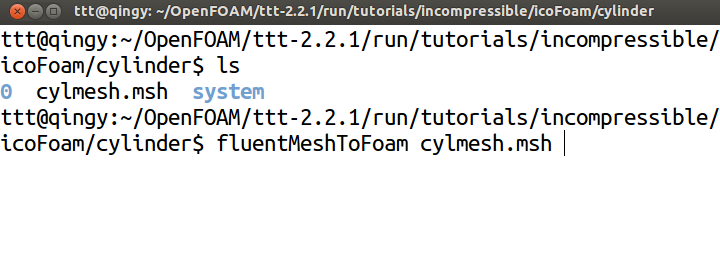
\includegraphics[width=\lgfig]{\LocCHonefivefig/conversion.png}
\caption{convert}
\label{mesh}
\end{figure}

\flushleft In case you have a 3D mesh file then you can use the command \\ \vspace{0.5cm}
\centering {\textbf{fluent3DMeshToFoam file-name.msh}} \newline

\flushleft The Fluent mesh file is converted into OpenFOAM mesh file. Now if we look back into our cylinder folder we can see that the "constant"
folder is now generated. When we open the constant folder we will see that the transport properties file is missing. Since we had converted the 
fluent mesh file into openfoam the fluid property files were missing. Copy the transport property file from the constant folder of cavity case
and paste this inside the constant folder of cylinder. The trasnportProperties file contains the value of fluid viscosity, we can either change it
or keep it default. \newline

\flushleft Make a note here that we do not use the \textbf{blockMesh} command here

\section{Boundary Conditions}

When we import the geometry in OpenFOAM we need to be very careful with the boudnary names used while creating the mesh file. Since OpenFOAM is case
sensitive in case of any mistake with the boundary names can create an error while running the solver. To view the boundary names in the command terminal
go to polyMesh folder inside the constant. Inside polyMesh you can see a file by the name \textbf{boundary}. Open this file in any editor of your
choice, eg, gedit boundary, Fig \ref{boundary}.

\begin{figure}[h]  
\centering
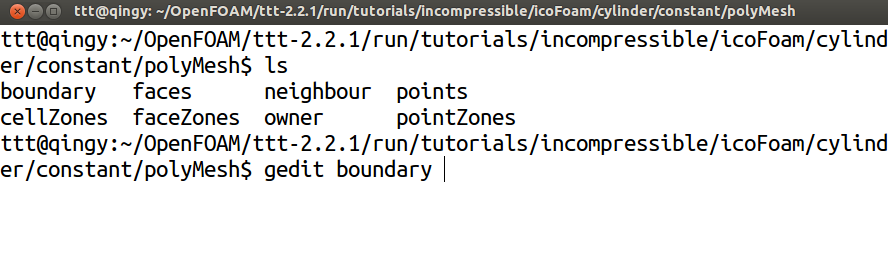
\includegraphics[width=\lgfig]{\LocCHonefivefig/boundary.png}
\caption{Boundary file}
\label{boundary}
\end{figure}

\flushleft The boundary names will be as shown in the domain shown above, Fig \ref{square}. In case of any error with the boundary names you can
always refer to this boundary file. Now in your command terminal go to the 0 folder and open the pressure file. Make sure that the boundary names 
match exactly the names in the boundary file, in case of errors make the necessary changes.

\section{Solver settings}

In the terminal window go to the controlDict file inside system and open it in any editor of your choice. Change the endTime from 0.5 to 1.5 seconds.
Save the file and close it, Fig \ref{cd} and come back to the cylinder folder.

\begin{figure}[h]  
\centering
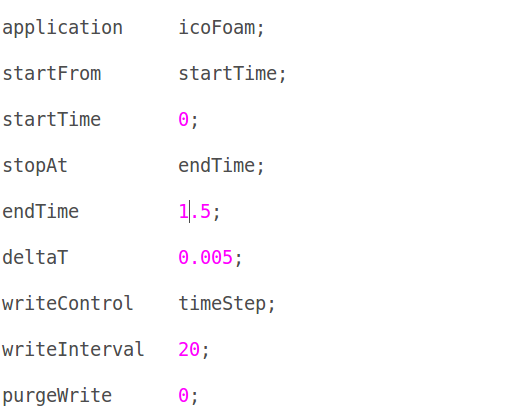
\includegraphics[width=\lgfig]{\LocCHonefivefig/controldict.png}
\caption{controlDict file}
\label{cd}
\end{figure}

\flushleft After making the necessary changes we can now run the solver. In the temrinal window type the name of the solver \textbf{icoFoam}
and press enter. The iterations will be seen running on the terminal window. After the iterations stop we can now start with the visualization.

\section{Post-Processing}

Launch paraview by typing \textbf{paraFoam} in the terminal window and once it opens click on the Apply button to view the geometry, Fig \ref{geom}.
In the active varialble control menu change from Solid Color to Velocity (U). You can now see the initial conditions for velocity, Fig \ref{vel}.
To view the animation on the right hand top of paraview click on the play button of VCR menu. You can see the change in velocity in the paraview 
window with the passage of time, Fig \ref {vel-1}.

\begin{figure}[h]  
\centering
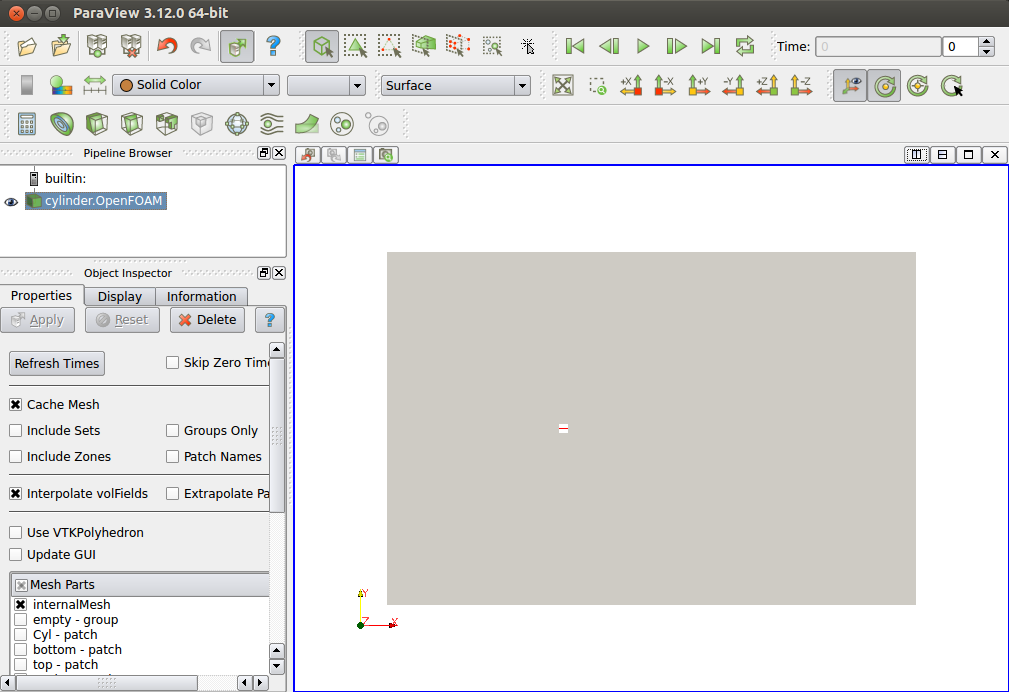
\includegraphics[width=\lgfig]{\LocCHonefivefig/geom-paraview.png}
\caption{Geometry in Paraview}
\label{geom}
\end{figure}

\begin{figure}[h]  
\centering
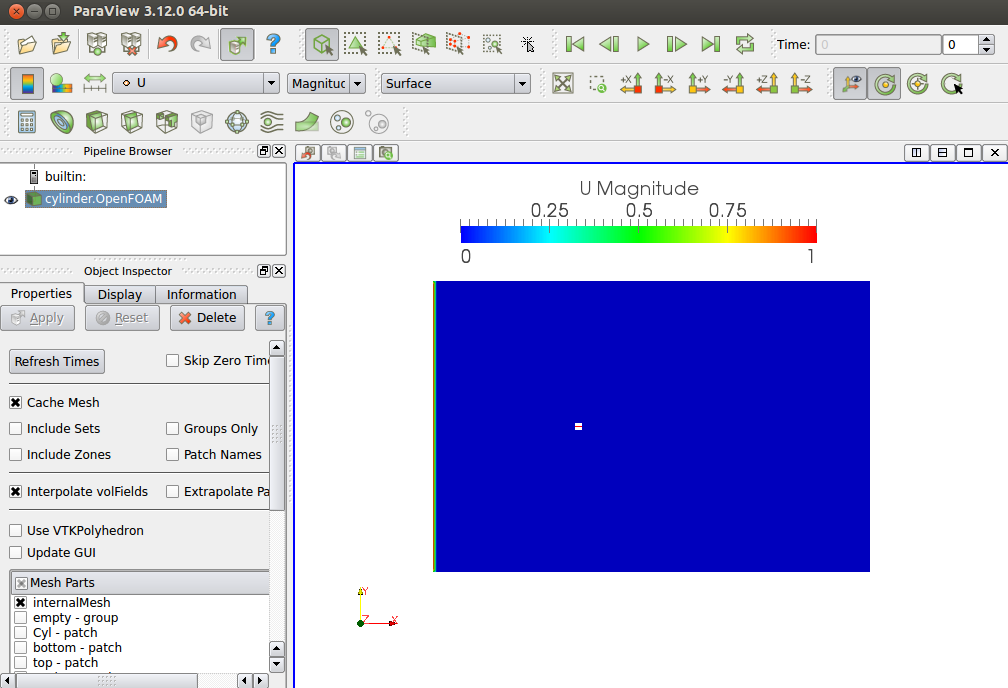
\includegraphics[width=\lgfig]{\LocCHonefivefig/vel.png}
\caption{Initial velocity condition}
\label{vel}
\end{figure}

\begin{figure}[h]  
\centering
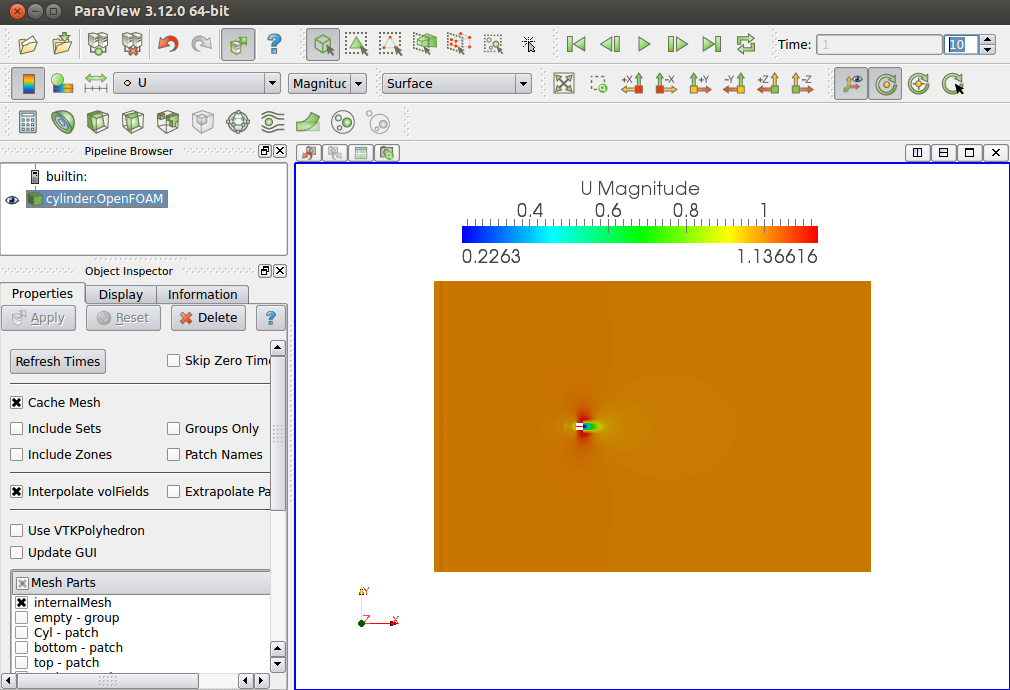
\includegraphics[width=\lgfig]{\LocCHonefivefig/vel-1.png}
\caption{Velocity at 1 sec}
\label{vel-1}
\end{figure}

\section{Mesh Conversion Commands}

The user can also import mesh files from other meshing softwares as well. Here is a list of commands to import mesh files in OpenFOAM.

\begin{itemize}
\item ANSYS : ansysToFoam file-name
\item IDEAS : ideasToFoam file-name
\item CFX : cfxToFoam file-name
\item SALOME : ideasUnvToFoam file-name
\end{itemize}


